% layout and global options
\documentclass
[
  draft    = true,
  fontsize = 11pt,
  parskip  = half-,
  BCOR     = 0pt,
  DIV      = 11,
  ngerman,
  dvipsnames
]
{scrartcl}

% default packages
\usepackage[utf8]{inputenc}
\usepackage[T1]{fontenc}
\usepackage{lmodern}
\usepackage{babel}
% extra packages
\usepackage{amsmath}
\usepackage{amssymb}
\usepackage{enumerate}
\usepackage{graphicx}
\usepackage{ifthen}
\usepackage{siunitx}
\usepackage{tikz}
\usepackage{url}
% own packages
\usepackage{mytemize}

% basic calculations in TikZ
\usetikzlibrary{calc}
\usetikzlibrary{decorations.pathreplacing}

% use comma as decimal separator
\sisetup{locale=DE, group-minimum-digits=4}

% common code
% -----
% achim
% -----
%
%
%
\newenvironment{achim}
{%
  \begingroup
    \par
    \color{Blue}%
}%
{%
  \endgroup
}%

% -------
% karsten
% -------
%
%
%
\newenvironment{karsten}
{%
  \begingroup
    \par
    \color{Red}%
}%
{%
  \endgroup
}%

% ------
% moritz
% ------
%
%
%
\newenvironment{moritz}
{%
  \begingroup
    \par
    \color{Green}%
}%
{%
  \endgroup
}%

% ----
% KV16
% ----
%
% This environment draws a 4x4 KV-map within a tikz environment.
%
\newenvironment{KV16}
{%
  % ----------------------------------------------------------------------------
  % Public functions                                            Public functions
  % ----------------------------------------------------------------------------
  % --------
  % nolabels
  % --------
  %
  % disable input labels
  %
  \newcommand{\nolabels}
  {%
    \renewcommand{\showlabels}{FALSE}%
  }%
  % ---------
  % noindices
  % ---------
  %
  % disable index numbers
  %
  \newcommand{\noindices}
  {%
    \renewcommand{\showindices}{FALSE}%
  }%
  % -----------
  % clearoutput
  % -----------
  %
  % empty all function values
  %
  \newcommand{\clearoutput}
  {%
    \setoutput{0}{}%
    \setoutput{1}{}%
    \setoutput{2}{}%
    \setoutput{3}{}%
    \setoutput{4}{}%
    \setoutput{5}{}%
    \setoutput{6}{}%
    \setoutput{7}{}%
    \setoutput{8}{}%
    \setoutput{9}{}%
    \setoutput{10}{}%
    \setoutput{11}{}%
    \setoutput{12}{}%
    \setoutput{13}{}%
    \setoutput{14}{}%
    \setoutput{15}{}%
  }%
  % --------
  % function
  % --------
  %
  % #1  name of the function
  %
  \newcommand{\function}[1]
  {%
    \renewcommand{\valuefname}{##1}%
  }%
  % ------
  % inputA
  % ------
  %
  % set the name of the input variable that toggles with the lowest frequency
  %
  % #1  name of the variable
  %
  \newcommand{\inputA}[1]
  {%
    \renewcommand{\valueinputA}{##1}%
  }%
  % ------
  % inputB
  % ------
  %
  % #1  name of the variable
  %
  \newcommand{\inputB}[1]
  {%
    \renewcommand{\valueinputB}{##1}%
  }%
  % ------
  % inputC
  % ------
  %
  % #1  name of the variable
  %
  \newcommand{\inputC}[1]
  {%
    \renewcommand{\valueinputC}{##1}%
  }%
  % ------
  % inputD
  % ------
  %
  % set the name of the input variable that toggles with the highest frequency
  %
  % #1  name of the variable
  %
  \newcommand{\inputD}[1]
  {%
    \renewcommand{\valueinputD}{##1}%
  }%
  % -------
  % minterm
  % -------
  %
  % #1  minterm number 0 ... 15
  %
  \newcommand{\minterm}[1]
  {%
    \setoutput{##1}{1}%
  }%
  % -------
  % maxterm
  % -------
  %
  % #1  maxterm number 0 ... 15
  %
  \newcommand{\maxterm}[1]
  {%
    \setoutput{##1}{0}%
  }%
  % --------
  % dontcare
  % --------
  %
  % #1  don't care number 0 ... 15
  %
  \newcommand{\dontcare}[1]
  {%
    \setoutput{##1}{X}%
  }%
  % -----
  % areas
  % -----
  %
  % define areas to fill
  %
  \newcommand{\areas}[1]
  {%
    \renewcommand{\printareas}{##1}
  }%
  % --------
  % colorize
  % --------
  %
  % #1 top row          (1..m)
  % #2 left column      (1..n)
  % #3 width            (number of columns)
  % #4 height           (number of rows)
  % #5 top    reduction (pt, cm, ...)
  % #6 bottom reduction (pt, cm, ...)
  % #7 left   reduction (pt, cm, ...)
  % #8 right  reduction (pt, cm, ...)
  % #9 color
  %
  \newcommand{\colorize}[9]
  {%
    \begin{scope}[xshift=0cm + (##2 - 1) * 1cm, yshift=4cm - (##1 - 1) * 1cm]
      % background
      \ifthenelse{\equal{\showtype}{FILL}}%
      {%
        \fill
        [
          opacity=0.5,
          fill=##9,
          rounded corners
        ] (0cm + ##7, 0cm - ##5) rectangle (1cm * ##3 - ##8, -1cm * ##4 + ##6);
      }%
      {\relax}%
      % border
      \ifthenelse{\equal{\showtype}{DRAW}}%
      {%
        \draw
        [
          draw=##9,
          line width=1pt,
          rounded corners
        ] (0cm + ##7, 0cm - ##5) rectangle (1cm * ##3 - ##8, -1cm * ##4 + ##6);
      }%
      {\relax}%
    \end{scope}
  }%
  % ----------------------------------------------------------------------------
  % Internal functions                                        Internal functions
  % ----------------------------------------------------------------------------
  % ---------
  % setoutput
  % ---------
  %
  % used my minterm, maxterm and dontcare
  %
  % #1  index: 0 .. 15
  % #2  text
  %
  \newcommand{\setoutput}[2]
  {%
    % map index to matrix position
    \ifthenelse{\equal{##1}{0}} {\renewcommand{\valueoutputAA}{##2}}{\relax}%
    \ifthenelse{\equal{##1}{1}} {\renewcommand{\valueoutputAB}{##2}}{\relax}%
    \ifthenelse{\equal{##1}{2}} {\renewcommand{\valueoutputAD}{##2}}{\relax}%
    \ifthenelse{\equal{##1}{3}} {\renewcommand{\valueoutputAC}{##2}}{\relax}%
    \ifthenelse{\equal{##1}{4}} {\renewcommand{\valueoutputBA}{##2}}{\relax}%
    \ifthenelse{\equal{##1}{5}} {\renewcommand{\valueoutputBB}{##2}}{\relax}%
    \ifthenelse{\equal{##1}{6}} {\renewcommand{\valueoutputBD}{##2}}{\relax}%
    \ifthenelse{\equal{##1}{7}} {\renewcommand{\valueoutputBC}{##2}}{\relax}%
    \ifthenelse{\equal{##1}{8}} {\renewcommand{\valueoutputDA}{##2}}{\relax}%
    \ifthenelse{\equal{##1}{9}} {\renewcommand{\valueoutputDB}{##2}}{\relax}%
    \ifthenelse{\equal{##1}{10}}{\renewcommand{\valueoutputDD}{##2}}{\relax}%
    \ifthenelse{\equal{##1}{11}}{\renewcommand{\valueoutputDC}{##2}}{\relax}%
    \ifthenelse{\equal{##1}{12}}{\renewcommand{\valueoutputCA}{##2}}{\relax}%
    \ifthenelse{\equal{##1}{13}}{\renewcommand{\valueoutputCB}{##2}}{\relax}%
    \ifthenelse{\equal{##1}{14}}{\renewcommand{\valueoutputCD}{##2}}{\relax}%
    \ifthenelse{\equal{##1}{15}}{\renewcommand{\valueoutputCC}{##2}}{\relax}%
  }%
  % -----------
  % printlabels
  % -----------
  %
  % print all input labels
  %
  \newcommand{\printlabels}
  {%
    \draw[|-|] ( 4.3,  0.0) -- node[right] {\valueinputA} ( 4.3,  2.0);
    \draw[|-|] (-0.3,  1.0) -- node[left]  {\valueinputB} (-0.3,  3.0);
    \draw[|-|] ( 1.0, -0.3) -- node[below] {\valueinputD} ( 3.0, -0.3);
    \draw[|-|] ( 2.0,  4.3) -- node[above] {\valueinputC} ( 4.0,  4.3);
  }%
  % ------------
  % printindices
  % ------------
  %
  % print all index numbers
  %
  \newcommand{\printindices}
  {%
    \begin{scope}[xshift=2mm, yshift=8mm]
      % 1. row (top)
      \node at (0, 3) {{\tiny\sffamily  0}};
      \node at (1, 3) {{\tiny\sffamily  1}};
      \node at (2, 3) {{\tiny\sffamily  3}};
      \node at (3, 3) {{\tiny\sffamily  2}};
      % 2. row
      \node at (0, 2) {{\tiny\sffamily  4}};
      \node at (1, 2) {{\tiny\sffamily  5}};
      \node at (2, 2) {{\tiny\sffamily  7}};
      \node at (3, 2) {{\tiny\sffamily  6}};
      % 3. row
      \node at (0, 1) {{\tiny\sffamily 12}};
      \node at (1, 1) {{\tiny\sffamily 13}};
      \node at (2, 1) {{\tiny\sffamily 15}};
      \node at (3, 1) {{\tiny\sffamily 14}};
      % 4. row (bottom)
      \node at (0, 0) {{\tiny\sffamily  8}};
      \node at (1, 0) {{\tiny\sffamily  9}};
      \node at (2, 0) {{\tiny\sffamily 11}};
      \node at (3, 0) {{\tiny\sffamily 10}};
    \end{scope}
  }%
  % -----------
  % printoutput
  % -----------
  %
  % show all output values
  %
  \newcommand{\printoutput}
  {%
    \begin{scope}[xshift=0.5cm, yshift=0.5cm]
      % 1. row (top)
      \node at (0, 3) {\valueoutputAA};
      \node at (1, 3) {\valueoutputAB};
      \node at (2, 3) {\valueoutputAC};
      \node at (3, 3) {\valueoutputAD};
      % 2. row
      \node at (0, 2) {\valueoutputBA};
      \node at (1, 2) {\valueoutputBB};
      \node at (2, 2) {\valueoutputBC};
      \node at (3, 2) {\valueoutputBD};
      % 3. row
      \node at (0, 1) {\valueoutputCA};
      \node at (1, 1) {\valueoutputCB};
      \node at (2, 1) {\valueoutputCC};
      \node at (3, 1) {\valueoutputCD};
      % 4. row (bottom)
      \node at (0, 0) {\valueoutputDA};
      \node at (1, 0) {\valueoutputDB};
      \node at (2, 0) {\valueoutputDC};
      \node at (3, 0) {\valueoutputDD};
    \end{scope}
  }%
  % ----------
  % printareas
  % ----------
  %
  % show all colorized areas
  %
  \newcommand{\printareas}{\relax}%
  % ----------------------------------------------------------------------------
  % Attributes                                                        Attributes
  % ----------------------------------------------------------------------------
  % some common colors
  \definecolor{C1}{named}{Red}%
  \definecolor{C2}{named}{Green}%
  \definecolor{C3}{named}{Blue}%
  \definecolor{C4}{named}{Sepia}%
  \definecolor{C5}{named}{Cyan}%
  \definecolor{C6}{named}{Magenta}%
  \definecolor{C7}{named}{Yellow}%
  \definecolor{C8}{named}{Gray}%
  % flags
  \newcommand{\showlabels}{TRUE}%
  \newcommand{\showindices}{TRUE}%
  % name of the function
  \newcommand{\valuefname}{\relax}%
  % names of the four input variables
  \newcommand{\valueinputA}{$e_3$}%
  \newcommand{\valueinputB}{$e_2$}%
  \newcommand{\valueinputC}{$e_1$}%
  \newcommand{\valueinputD}{$e_0$}%
  % output values (matrix positions)
  \newcommand{\valueoutputAA}{0}% 0
  \newcommand{\valueoutputAB}{0}% 1
  \newcommand{\valueoutputAC}{0}% 3
  \newcommand{\valueoutputAD}{0}% 2
  \newcommand{\valueoutputBA}{0}% 4
  \newcommand{\valueoutputBB}{0}% 5
  \newcommand{\valueoutputBC}{0}% 7
  \newcommand{\valueoutputBD}{0}% 6
  \newcommand{\valueoutputCA}{0}% 12
  \newcommand{\valueoutputCB}{0}% 13
  \newcommand{\valueoutputCC}{0}% 15
  \newcommand{\valueoutputCD}{0}% 14
  \newcommand{\valueoutputDA}{0}% 8
  \newcommand{\valueoutputDB}{0}% 9
  \newcommand{\valueoutputDC}{0}% 11
  \newcommand{\valueoutputDD}{0}% 10
}%
{%
  \begingroup
    % show colored areas first (lowest layer)
    \begin{scope}
      % clip colored areas
      \clip (-0.15, -0.15) rectangle (4.15, 4.15);
      % show background
      {\newcommand{\showtype}{FILL}\printareas}%
      % show border
      {\newcommand{\showtype}{DRAW}\printareas}%
    \end{scope}
    % show grid
    \draw (0, 0) grid (4, 4);
    % name of the function
    \ifthenelse{\equal{\valuefname}{\relax}}{\relax}{\node at (-0.5, 4.5) {\valuefname};}
    % labels
    \ifthenelse{\equal{\showlabels}{TRUE}}{\printlabels}{\relax}
    % indices
    \ifthenelse{\equal{\showindices}{TRUE}}{\printindices}{\relax}
    % output values
    \printoutput
  \endgroup
}%

% ----
% KV32
% ----
%
% This environment draws a 4x8 KV-map within a tikz environment.
%
\newenvironment{KV32}
{%
  % ----------------------------------------------------------------------------
  % Public functions                                            Public functions
  % ----------------------------------------------------------------------------
  % --------
  % nolabels
  % --------
  %
  % disable input labels
  %
  \newcommand{\nolabels}
  {%
    \renewcommand{\showlabels}{FALSE}%
  }%
  % ---------
  % noindices
  % ---------
  %
  % disable index numbers
  %
  \newcommand{\noindices}
  {%
    \renewcommand{\showindices}{FALSE}%
  }%
  % -----------
  % clearoutput
  % -----------
  %
  % empty all function values
  %
  \newcommand{\clearoutput}
  {%
    \setoutput{0}{}%
    \setoutput{1}{}%
    \setoutput{2}{}%
    \setoutput{3}{}%
    \setoutput{4}{}%
    \setoutput{5}{}%
    \setoutput{6}{}%
    \setoutput{7}{}%
    \setoutput{8}{}%
    \setoutput{9}{}%
    \setoutput{10}{}%
    \setoutput{11}{}%
    \setoutput{12}{}%
    \setoutput{13}{}%
    \setoutput{14}{}%
    \setoutput{15}{}%
    \setoutput{16}{}%
    \setoutput{17}{}%
    \setoutput{18}{}%
    \setoutput{19}{}%
    \setoutput{20}{}%
    \setoutput{21}{}%
    \setoutput{22}{}%
    \setoutput{23}{}%
    \setoutput{24}{}%
    \setoutput{25}{}%
    \setoutput{26}{}%
    \setoutput{27}{}%
    \setoutput{28}{}%
    \setoutput{29}{}%
    \setoutput{30}{}%
    \setoutput{31}{}%
  }%
  % --------
  % function
  % --------
  %
  % #1  name of the function
  %
  \newcommand{\function}[1]
  {%
    \renewcommand{\valuefname}{##1}%
  }%
  % ------
  % inputA
  % ------
  %
  % set the name of the input variable that toggles with the lowest frequency
  %
  % #1  name of the variable
  %
  \newcommand{\inputA}[1]
  {%
    \renewcommand{\valueinputA}{##1}%
  }%
  % ------
  % inputB
  % ------
  %
  % #1  name of the variable
  %
  \newcommand{\inputB}[1]
  {%
    \renewcommand{\valueinputB}{##1}%
  }%
  % ------
  % inputC
  % ------
  %
  % #1  name of the variable
  %
  \newcommand{\inputC}[1]
  {%
    \renewcommand{\valueinputC}{##1}%
  }%
  % ------
  % inputD
  % ------
  %
  % #1  name of the variable
  %
  \newcommand{\inputD}[1]
  {%
    \renewcommand{\valueinputD}{##1}%
  }%
  % ------
  % inputE
  % ------
  %
  % set the name of the input variable that toggles with the highest frequency
  %
  % #1  name of the variable
  %
  \newcommand{\inputE}[1]
  {%
    \renewcommand{\valueinputE}{##1}%
  }%
  % -------
  % minterm
  % -------
  %
  % #1  minterm number 0 ... 31
  %
  \newcommand{\minterm}[1]
  {%
    \setoutput{##1}{1}%
  }%
  % -------
  % maxterm
  % -------
  %
  % #1  maxterm number 0 ... 31
  %
  \newcommand{\maxterm}[1]
  {%
    \setoutput{##1}{0}%
  }%
  % --------
  % dontcare
  % --------
  %
  % #1  don't care number 0 ... 31
  %
  \newcommand{\dontcare}[1]
  {%
    \setoutput{##1}{X}%
  }%
  % -----
  % areas
  % -----
  %
  % define areas to fill
  %
  \newcommand{\areas}[1]
  {%
    \renewcommand{\printareas}{##1}
  }%
  % --------
  % colorize
  % --------
  %
  % #1 top row          (1..m)
  % #2 left column      (1..n)
  % #3 width            (number of columns)
  % #4 height           (number of rows)
  % #5 top    reduction (pt, cm, ...)
  % #6 bottom reduction (pt, cm, ...)
  % #7 left   reduction (pt, cm, ...)
  % #8 right  reduction (pt, cm, ...)
  % #9 color
  %
  \newcommand{\colorize}[9]
  {%
    \begin{scope}[xshift=0cm + (##2 - 1) * 1cm, yshift=4cm - (##1 - 1) * 1cm]
      % background
      \ifthenelse{\equal{\showtype}{FILL}}%
      {%
        \fill
        [
          opacity=0.5,
          fill=##9,
          rounded corners
        ] (0cm + ##7, 0cm - ##5) rectangle (1cm * ##3 - ##8, -1cm * ##4 + ##6);
      }%
      {\relax}%
      % border
      \ifthenelse{\equal{\showtype}{DRAW}}%
      {%
        \draw
        [
          draw=##9,
          line width=1pt,
          rounded corners
        ] (0cm + ##7, 0cm - ##5) rectangle (1cm * ##3 - ##8, -1cm * ##4 + ##6);
      }%
      {\relax}%
    \end{scope}
  }%
  % ----------------------------------------------------------------------------
  % Internal functions                                        Internal functions
  % ----------------------------------------------------------------------------
  % ---------
  % setoutput
  % ---------
  %
  % used my minterm, maxterm and dontcare
  %
  % #1  index: 0 .. 31
  % #2  text
  %
  \newcommand{\setoutput}[2]
  {%
    % map index to matrix position
    \ifthenelse{\equal{##1}{0}} {\renewcommand{\valueoutputAA}{##2}}{\relax}%
    \ifthenelse{\equal{##1}{1}} {\renewcommand{\valueoutputAB}{##2}}{\relax}%
    \ifthenelse{\equal{##1}{2}} {\renewcommand{\valueoutputAD}{##2}}{\relax}%
    \ifthenelse{\equal{##1}{3}} {\renewcommand{\valueoutputAC}{##2}}{\relax}%
    \ifthenelse{\equal{##1}{4}} {\renewcommand{\valueoutputBA}{##2}}{\relax}%
    \ifthenelse{\equal{##1}{5}} {\renewcommand{\valueoutputBB}{##2}}{\relax}%
    \ifthenelse{\equal{##1}{6}} {\renewcommand{\valueoutputBD}{##2}}{\relax}%
    \ifthenelse{\equal{##1}{7}} {\renewcommand{\valueoutputBC}{##2}}{\relax}%
    \ifthenelse{\equal{##1}{8}} {\renewcommand{\valueoutputDA}{##2}}{\relax}%
    \ifthenelse{\equal{##1}{9}} {\renewcommand{\valueoutputDB}{##2}}{\relax}%
    \ifthenelse{\equal{##1}{10}}{\renewcommand{\valueoutputDD}{##2}}{\relax}%
    \ifthenelse{\equal{##1}{11}}{\renewcommand{\valueoutputDC}{##2}}{\relax}%
    \ifthenelse{\equal{##1}{12}}{\renewcommand{\valueoutputCA}{##2}}{\relax}%
    \ifthenelse{\equal{##1}{13}}{\renewcommand{\valueoutputCB}{##2}}{\relax}%
    \ifthenelse{\equal{##1}{14}}{\renewcommand{\valueoutputCD}{##2}}{\relax}%
    \ifthenelse{\equal{##1}{15}}{\renewcommand{\valueoutputCC}{##2}}{\relax}%
    \ifthenelse{\equal{##1}{16}}{\renewcommand{\valueoutputAH}{##2}}{\relax}%
    \ifthenelse{\equal{##1}{17}}{\renewcommand{\valueoutputAG}{##2}}{\relax}%
    \ifthenelse{\equal{##1}{18}}{\renewcommand{\valueoutputAE}{##2}}{\relax}%
    \ifthenelse{\equal{##1}{19}}{\renewcommand{\valueoutputAF}{##2}}{\relax}%
    \ifthenelse{\equal{##1}{20}}{\renewcommand{\valueoutputBH}{##2}}{\relax}%
    \ifthenelse{\equal{##1}{21}}{\renewcommand{\valueoutputBG}{##2}}{\relax}%
    \ifthenelse{\equal{##1}{22}}{\renewcommand{\valueoutputBE}{##2}}{\relax}%
    \ifthenelse{\equal{##1}{23}}{\renewcommand{\valueoutputBF}{##2}}{\relax}%
    \ifthenelse{\equal{##1}{24}}{\renewcommand{\valueoutputDH}{##2}}{\relax}%
    \ifthenelse{\equal{##1}{25}}{\renewcommand{\valueoutputDG}{##2}}{\relax}%
    \ifthenelse{\equal{##1}{26}}{\renewcommand{\valueoutputDE}{##2}}{\relax}%
    \ifthenelse{\equal{##1}{27}}{\renewcommand{\valueoutputDF}{##2}}{\relax}%
    \ifthenelse{\equal{##1}{28}}{\renewcommand{\valueoutputCH}{##2}}{\relax}%
    \ifthenelse{\equal{##1}{29}}{\renewcommand{\valueoutputCG}{##2}}{\relax}%
    \ifthenelse{\equal{##1}{30}}{\renewcommand{\valueoutputCE}{##2}}{\relax}%
    \ifthenelse{\equal{##1}{31}}{\renewcommand{\valueoutputCF}{##2}}{\relax}%
  }%
  % -----------
  % printlabels
  % -----------
  %
  % print all input labels
  %
  \newcommand{\printlabels}
  {%
    \draw[|-|] ( 8.3,  0.0) -- node[right] {\valueinputB} ( 8.3,  2.0);
    \draw[|-|] (-0.3,  1.0) -- node[left]  {\valueinputC} (-0.3,  3.0);
    \draw[|-|] ( 1.0, -0.3) -- node[below] {\valueinputE} ( 3.0, -0.3);
    \draw[|-|] ( 5.0, -0.3) -- node[below] {\valueinputE} ( 7.0, -0.3);
    \draw[|-|] ( 2.0,  4.3) -- node[above] {\valueinputD} ( 6.0,  4.3);
    \draw[|-|] ( 4.0,  5.0) -- node[above] {\valueinputA} ( 8.0,  5.0);
  }%
  % ------------
  % printindices
  % ------------
  %
  % print all index numbers
  %
  \newcommand{\printindices}
  {%
    \begin{scope}[xshift=2mm, yshift=8mm]
      % 1. row (top)
      \node at (0, 3) {{\tiny\sffamily  0}};
      \node at (1, 3) {{\tiny\sffamily  1}};
      \node at (2, 3) {{\tiny\sffamily  3}};
      \node at (3, 3) {{\tiny\sffamily  2}};
      \node at (4, 3) {{\tiny\sffamily 18}};
      \node at (5, 3) {{\tiny\sffamily 19}};
      \node at (6, 3) {{\tiny\sffamily 17}};
      \node at (7, 3) {{\tiny\sffamily 16}};
      % 2. row
      \node at (0, 2) {{\tiny\sffamily  4}};
      \node at (1, 2) {{\tiny\sffamily  5}};
      \node at (2, 2) {{\tiny\sffamily  7}};
      \node at (3, 2) {{\tiny\sffamily  6}};
      \node at (4, 2) {{\tiny\sffamily 22}};
      \node at (5, 2) {{\tiny\sffamily 23}};
      \node at (6, 2) {{\tiny\sffamily 21}};
      \node at (7, 2) {{\tiny\sffamily 20}};
      % 3. row
      \node at (0, 1) {{\tiny\sffamily 12}};
      \node at (1, 1) {{\tiny\sffamily 13}};
      \node at (2, 1) {{\tiny\sffamily 15}};
      \node at (3, 1) {{\tiny\sffamily 14}};
      \node at (4, 1) {{\tiny\sffamily 30}};
      \node at (5, 1) {{\tiny\sffamily 31}};
      \node at (6, 1) {{\tiny\sffamily 29}};
      \node at (7, 1) {{\tiny\sffamily 28}};
      % 4. row (bottom)
      \node at (0, 0) {{\tiny\sffamily  8}};
      \node at (1, 0) {{\tiny\sffamily  9}};
      \node at (2, 0) {{\tiny\sffamily 11}};
      \node at (3, 0) {{\tiny\sffamily 10}};
      \node at (4, 0) {{\tiny\sffamily 26}};
      \node at (5, 0) {{\tiny\sffamily 27}};
      \node at (6, 0) {{\tiny\sffamily 25}};
      \node at (7, 0) {{\tiny\sffamily 24}};
    \end{scope}
  }%
  % -----------
  % printoutput
  % -----------
  %
  % show all output values
  %
  \newcommand{\printoutput}
  {%
    \begin{scope}[xshift=0.5cm, yshift=0.5cm]
      % 1. row (top)
      \node at (0, 3) {\valueoutputAA};
      \node at (1, 3) {\valueoutputAB};
      \node at (2, 3) {\valueoutputAC};
      \node at (3, 3) {\valueoutputAD};
      \node at (4, 3) {\valueoutputAE};
      \node at (5, 3) {\valueoutputAF};
      \node at (6, 3) {\valueoutputAG};
      \node at (7, 3) {\valueoutputAH};
      % 2. row
      \node at (0, 2) {\valueoutputBA};
      \node at (1, 2) {\valueoutputBB};
      \node at (2, 2) {\valueoutputBC};
      \node at (3, 2) {\valueoutputBD};
      \node at (4, 2) {\valueoutputBE};
      \node at (5, 2) {\valueoutputBF};
      \node at (6, 2) {\valueoutputBG};
      \node at (7, 2) {\valueoutputBH};
      % 3. row
      \node at (0, 1) {\valueoutputCA};
      \node at (1, 1) {\valueoutputCB};
      \node at (2, 1) {\valueoutputCC};
      \node at (3, 1) {\valueoutputCD};
      \node at (4, 1) {\valueoutputCE};
      \node at (5, 1) {\valueoutputCF};
      \node at (6, 1) {\valueoutputCG};
      \node at (7, 1) {\valueoutputCH};
      % 4. row (bottom)
      \node at (0, 0) {\valueoutputDA};
      \node at (1, 0) {\valueoutputDB};
      \node at (2, 0) {\valueoutputDC};
      \node at (3, 0) {\valueoutputDD};
      \node at (4, 0) {\valueoutputDE};
      \node at (5, 0) {\valueoutputDF};
      \node at (6, 0) {\valueoutputDG};
      \node at (7, 0) {\valueoutputDH};
    \end{scope}
  }%
  % ----------
  % printareas
  % ----------
  %
  % show all colorized areas
  %
  \newcommand{\printareas}{\relax}%
  % ----------------------------------------------------------------------------
  % Attributes                                                        Attributes
  % ----------------------------------------------------------------------------
  % some common colors
  \definecolor{C1}{named}{Red}%
  \definecolor{C2}{named}{Green}%
  \definecolor{C3}{named}{Blue}%
  \definecolor{C4}{named}{Sepia}%
  \definecolor{C5}{named}{Cyan}%
  \definecolor{C6}{named}{Magenta}%
  \definecolor{C7}{named}{Yellow}%
  \definecolor{C8}{named}{Gray}%
  % flags
  \newcommand{\showlabels}{TRUE}%
  \newcommand{\showindices}{TRUE}%
  % name of the function
  \newcommand{\valuefname}{\relax}%
  % names of the five input variables
  \newcommand{\valueinputA}{$e_4$}%
  \newcommand{\valueinputB}{$e_3$}%
  \newcommand{\valueinputC}{$e_2$}%
  \newcommand{\valueinputD}{$e_1$}%
  \newcommand{\valueinputE}{$e_0$}%
  % output values (matrix positions)
  \newcommand{\valueoutputAA}{$0$}% 0
  \newcommand{\valueoutputAB}{$0$}% 1
  \newcommand{\valueoutputAC}{$0$}% 3
  \newcommand{\valueoutputAD}{$0$}% 2
  \newcommand{\valueoutputAE}{$0$}% 18
  \newcommand{\valueoutputAF}{$0$}% 19
  \newcommand{\valueoutputAG}{$0$}% 17
  \newcommand{\valueoutputAH}{$0$}% 16
  \newcommand{\valueoutputBA}{$0$}% 4
  \newcommand{\valueoutputBB}{$0$}% 5
  \newcommand{\valueoutputBC}{$0$}% 7
  \newcommand{\valueoutputBD}{$0$}% 6
  \newcommand{\valueoutputBE}{$0$}% 22
  \newcommand{\valueoutputBF}{$0$}% 23
  \newcommand{\valueoutputBG}{$0$}% 21
  \newcommand{\valueoutputBH}{$0$}% 20
  \newcommand{\valueoutputCA}{$0$}% 12
  \newcommand{\valueoutputCB}{$0$}% 13
  \newcommand{\valueoutputCC}{$0$}% 15
  \newcommand{\valueoutputCD}{$0$}% 14
  \newcommand{\valueoutputCE}{$0$}% 30
  \newcommand{\valueoutputCF}{$0$}% 31
  \newcommand{\valueoutputCG}{$0$}% 29
  \newcommand{\valueoutputCH}{$0$}% 28
  \newcommand{\valueoutputDA}{$0$}% 8
  \newcommand{\valueoutputDB}{$0$}% 9
  \newcommand{\valueoutputDC}{$0$}% 11
  \newcommand{\valueoutputDD}{$0$}% 10
  \newcommand{\valueoutputDE}{$0$}% 26
  \newcommand{\valueoutputDF}{$0$}% 27
  \newcommand{\valueoutputDG}{$0$}% 25
  \newcommand{\valueoutputDH}{$0$}% 24
}%
{%
  \begingroup
    % show colored areas first (lowest layer)
    \begin{scope}
      % clip colored areas
      \clip (-0.15, -0.15) rectangle (8.15, 4.15);
      % show background
      {\newcommand{\showtype}{FILL}\printareas}%
      % show border
      {\newcommand{\showtype}{DRAW}\printareas}%
    \end{scope}
    % show grid
    \draw (0, 0) grid (8, 4);
    % name of the function
    \ifthenelse{\equal{\valuefname}{\relax}}{\relax}{\node at (-0.5, 4.5) {\valuefname};}
    % labels
    \ifthenelse{\equal{\showlabels}{TRUE}}{\printlabels}{\relax}
    % indices
    \ifthenelse{\equal{\showindices}{TRUE}}{\printindices}{\relax}
    % output values
    \printoutput
  \endgroup
}%


% ------------------------------------------------------------------------------
\begin{document}
% ------------------------------------------------------------------------------

% --------------------------------------------------------------
\section*{Digitaltechnik und Rechnerorganisation: Fragenkatalog}
% --------------------------------------------------------------

% github repository
\url{https://github.com/usishare/DuR_WS1819_Fragenkatalog.git}

\newsavebox{\tempbox}%

% ----------------------
\subsection*{Grundlagen}
% ----------------------
\begin{mytemize}
  \item Was besagt das Mooresche Gesetz? 
        \begin{achim}
          \begin{mytemize}
            \item Verdopplung der Anzahl von Transitoren pro Fläche alle zwei Jahre
          \end{mytemize}
        \end{achim}
  \item Erklären Sie das \glqq{}Design-Technology-Gap\grqq. 
        \begin{achim}
          \begin{mytemize}
            \item Die tatsächliche Leistungszunahme digitaler Systeme folgt nicht dem Mooreschen Gesetz,
                  sondern bleibt dahinter zurück.
            \item Die Weiterentwicklung der Software-Entwicklungswerkzeuge hält mit der
                  Verdopplung der Anzahl der Transistoren nicht Schritt.
          \end{mytemize}
        \end{achim}
  \item Nennen Sie die Abstraktionsebenen (Hardware und Software) bei der Entwicklung digitaler Systeme. 
        \begin{achim}
          \begin{center}
            \begin{tikzpicture}
              \newcommand{\nodebox}[2]
              {%
                \begin{scope}[shift={#1}]
                  \draw[line width=0.6pt] (-6em, -4mm) rectangle (6em, 4mm);
                  \node at (0, 0) {#2};
                \end{scope}%
              }%
              \nodebox{(0,  3.5)}{Algorithmen}
              \nodebox{(0,  2.5)}{Betriebssystemebene}
              \nodebox{(0,  1.5)}{Assembler}
              \nodebox{(0,  0.5)}{Maschinensprache}
              \nodebox{(0, -0.5)}{Mikroarchitektur}
              \nodebox{(0, -1.5)}{Digitale Logik}
              \nodebox{(0, -2.5)}{Transistoren}
              \nodebox{(0, -3.5)}{IC Processing / Physik}
              \draw[line width=0.6pt, decorate, decoration=brace] (-7em, -3.9) -- node[left=1mm]{Hardware} (-7em, -0.1);
              \draw[line width=0.6pt, decorate, decoration=brace] (-7em,  0.1) -- node[left=1mm]{Software} (-7em,  3.9);
              \draw[line width=0.6pt, decorate, decoration=brace] ( 7em, -0.1) -- node[right=1mm]{DuR}     ( 7em, -2.0);
            \end{tikzpicture}
          \end{center}
        \end{achim}
  \item Erklären Sie die Begriffe \glqq{}digital\grqq{} und \glqq{}analog\grqq{} sowie \glqq{}zeitdiskret\grqq{} und \glqq{}zeitkontinuierlich\grqq. Geben Sie Beispiele. 
        \begin{achim}
          \begin{mytemize}
            \item analog: im Rahmen der Signaltheorie ist ein analoges Signal ein Signal mit stufenlosem und unterbrechungsfreiem Verlauf
            \item digital: im Rahmen der Signaltheorie ist ein digitales Signal ein Signal, das nur einen abgegrenzten und gestuften Wertvorrat umfasst
          \end{mytemize}
        \end{achim}
        \begin{moritz}
        \begin{itemize}
                \item[]\textbf{zeitdiskret:} Signal ist nur zu bestimmten Zeitpunkten definiert (z.\,B. 0, 1). Kein durchgehender Zeitverlauf.
        \end{itemize}
        \end{moritz}
  \item Wie funktioniert die Digitalisierung eines Signals? 
        \begin{achim}
          \begin{mytemize}
            \item Abtastung
            \item Quantisierung
          \end{mytemize}
        \end{achim}
  \item Was ist das Abtasttheorem? 
        \begin{achim}
          \begin{mytemize}
            \item Abtastfrequenz muss mindestens doppelt so groß sein wie die obere Grenzfrequenz des Signals
          \end{mytemize}
        \end{achim}
  \item Was sind Quantisierungsfehler und Aliasing? 
        \begin{achim}
          \begin{mytemize}
            \item Quantisierungsfehler entstehen durch die unterschiedliche Anzahl von Bits, die pro Abtastwert zur Verfügung stehen
            \item Aliasing bewirkt bei zu geringer Abtastrate, dass zu hohe Frequenzen als tiefere Frequenzen auftauchen
          \end{mytemize}
        \end{achim}
  \item Was sind digitale Logikpegel und wozu dienen sie? 
        \begin{achim}
          \begin{mytemize}
            \item Nur zwei -- nicht zusammenhängende -- Bereiche im Wertebereich eines Signals
                  tragen eine Bedeutung (0 bzw. 1). Im Vergleich zu analogen Pegeln steigt  
                  dadurch die Robustheit gegenüber Rauschen.
          \end{mytemize}
        \end{achim}
\end{mytemize}

% -------------------------------
\subsection*{Zahlendarstellungen}
% -------------------------------
\begin{mytemize}
  \item Wie funktioniert die Konversion einer Binärzahl in eine Dezimalzahl?
        \begin{achim}
          \begin{equation*}
            x_2=d_n\ldots d_1d_0
            \quad\Rightarrow\quad
            x_{10}=\sum_{i=0}^{n}d_i\cdot2^i
          \end{equation*}
        \end{achim}
        \begin{moritz}
        	\item[] \textbf{Binär zu Dezimal:} Man multipliziert die einzelnen Binärzahlen mit 2 hoch dem Stellenwert der Binärzahl.
          \item[] Zum Beispiel: 1010$\rightarrow$ $1*2^3+0*2^2+1*2^1+0*2^0=10$
        \end{moritz}
  \item Wie funktioniert die Konversion einer Dezimalzahl in eine Binärzahl?
  \begin{moritz}
    \begin{mytemize}
  	\item[] \textbf{Dezimal zu Binär:} Die Dezimal wird durch 2 mit Rest geteilt.
            Man teilt dann das geteilte durch wieder durch 2 mit Rest bis man 1 durch 2 geteilt hat.
            Der Rest der Division bildet die Binärzahl von Unten nach oben gelesen.
    \item[] Zum Beispiel: 11$\rightarrow$1101
      \begin{center}
        \setlength{\tabcolsep}{4ex}
        \begin{tabular}{|l|l|l|l|}
          \hline
          Schritte & Divison & Ergebenis & Rest \\ \hline
          1 & 11/2 & 5 & 1 \\ \hline
          2 & 5/2 & 2 & 1 \\ \hline
          3 & 2/2 & 1 & 0 \\ \hline
          4 & 1/2 & 0 & 1 \\ \hline
        \end{tabular}
      \end{center}
    \end{mytemize}
  \end{moritz}
  \item Wie können negative Zahlen repräsentiert werden und was sind die Eigenschaften der Darstellungen?
        \begin{achim}
          \begin{mytemize}
            \item Signierte Zahlendarstellung
                  \begin{mytemize}
                    \item der Absolutbetrag der Zahl wird zur Basis 2 dargestellt
                    \item das führende Bit signalisiert mit dem Wert 1 ein negatives Vorzeichen
                    \item die Zahl 0 besitzt mit $+0$ und $-0$ zwei verschiedene Darstellungen
                    \item für die Addition und die Subtraktion werden zwei verschiedene Schaltungen benötigt
                    \item der Additionsalgorithmuss benötigt eine Fallunterscheidung bezüglich des Vorzeichens der beiden Operanden
                  \end{mytemize}
            \item Einerkomplement-Darstellung
                  \begin{mytemize}
                    \item negative Zahlen werden nicht durch ein führendes Vorzeichenbit gekennzeichnet,
                          sondern dadurch, dass alle Bits invertiert werden
                    \item positive Zahlen können immer noch an einer führenden Null erkannt werden
                    \item für die 0 gibt es leider immer noch zwei verschiedene Darstellungen: $0\ldots0$ und $1\ldots1$
                    \item der Additionsalgorithmus funktioniert hier ohne Fallunterscheidung
                    \item die Überschreitung der 0 muss allerdings berücksichtigt werden (weil sie zweimal vorhanden ist)
                  \end{mytemize}
            \item Zweierkomplement-Darstellung
                  \begin{mytemize}
                    \item man erhält ein geschlossenes Zahlensystem mit $2^n$ verschiedenen Werten von $-2^{n-1}$ bis $2^{n-1}-1$
                    \item das höchstwertige Bit der Binärzahl steht nicht für $2^n$, sondern für $-2^n$
                          \begin{equation*}
                            1010=1\cdot-2^3+0\cdot2^2+1\cdot2^1+0\cdot2^0=-8+2=-6
                          \end{equation*}
                    \item man erhält die Zweierkomplement-Darstellung einer Zahl zum Beispiel, indem man zu ihrer
                          Einerkomplement-Darstellung die Zahl 1 addiert
                    \item die Zahl 0 besitzt eine eindeutige Darstellung
                    \item es kann ohne Fallunterscheidungen und Sondefälle addiert werden
                  \end{mytemize}
          \end{mytemize}
        \end{achim}
\end{mytemize}

% -----------------------------
\subsection*{Boolesche Algebra}
% -----------------------------
\begin{mytemize}
  \item Was ist ein
        \begin{mytemize}
          \item neutrales Element?
	          \begin{mytemize}
	          	\begin{karsten}
	          		\item Das neutrale Element hat keine Auswirkungen auf das Ergebnis der Verknüpfung
	          		\item $a \circ N = a$
	          	\end{karsten}
        \end{mytemize}
          \item inverses Element?
	          \begin{mytemize}
		          \begin{karsten}
		          	\item Eine Verknüpfung mit dem Inversen Element resultiert im neutralen Element
		          	\item $a \circ a^{-1} = N$
		          \end{karsten}
	          \end{mytemize}
        \end{mytemize}
  \item Erklären Sie
        \begin{mytemize}
          \item Abgeschlossenheit
                \begin{achim}
                  \begin{mytemize}
                    \item Eine zweistellige Operation $\circ$ ist bezüglich einer Menge $M$ abgeschlossen,
                          wenn alle ihre Ergebnisse wieder in $M$ liegen:
                          \begin{equation*}
                            \forall\;a,b\in M\quad\Rightarrow\quad(a\circ b)\in M
                          \end{equation*}
                  \end{mytemize}
                \end{achim}
          \item Assoziativgesetz
                \begin{achim}
                  \begin{mytemize}
                    \item Eine zweistellige Operation $\circ$ heißt assoziativ, wenn das Ergebnis
                          nicht von der Reihenfolge der Ausführung abhängig ist:
                          \begin{equation*}
                            (a\circ b)\circ c=a\circ(b\circ c)
                          \end{equation*}
                  \end{mytemize}
                \end{achim}
          \item Kommutativgesetz
                \begin{achim}
                  \begin{mytemize}
                    \item Eine zweistellige Operation $\circ$ heißt kommutativ, wenn das Ergebnis
                          nicht von der Reihenfolge der Operanden anhängig ist:
                          \begin{equation*}
                            a\circ b=b\circ a
                          \end{equation*}
                  \end{mytemize}
                \end{achim}
          \item Distributivgesetz
                \begin{achim}
                  \begin{mytemize}
                    \item Das Distributivgesetz legt fest, wie sich zwei zweistellige Operationen
                          bei der Auflösung von Klammern zueinmander verhalten:
                          \begin{equation*}
                            a\otimes(b\oplus c)=a\otimes b\oplus a\otimes c
                          \end{equation*}
                  \end{mytemize}
                \end{achim}
        \end{mytemize}
  \item Was sind die Axiome einer Booleschen Algebra?
        \begin{achim}
          Eine Menge $B$ mit zwei zweistelligen Operationen $\oplus$ und $\otimes$
          heißt genau dann \emph{Boolesche Algebra}, wenn folgende Axiome gelten:
          \begin{mytemize}
            \item Abgeschlossenheit bezüglich $\oplus$
            \item Abgeschlossenheit bezüglich $\otimes$
            \item Neutrales Element bezüglich $\oplus$: $(N)$ull
            \item Neutrales Element bezüglich $\otimes$: $(E)$ins
            \item $\oplus$ ist kommutativ
            \item $\otimes$ ist kommutativ
            \item $\oplus$ ist distributiv über $\otimes$
                  \begin{equation*}
                    a\oplus(b\otimes c)=a\oplus b\otimes a\oplus c
                  \end{equation*}
            \item $\otimes$ ist distributiv über $\oplus$
                  \begin{equation*}
                    a\otimes(b\oplus c)=a\otimes b\oplus a\otimes c
                  \end{equation*}
            \item Falls $N$ und $E$ existieren und eindeutig sind,
                  dann gibt es für jedes Element $a\in B$ ein Element $\bar{a}\in B$
                  (genannt Komplement) mit
                  \begin{equation*}
                    a\oplus\bar{a}=E
                    \qquad\text{und}\qquad
                    a\otimes\bar{a}=N
                  \end{equation*}
            \item es gibt mindestens zwei Elemente $a,b\in B$, für die $a\neq b$ gilt
          \end{mytemize}
        \end{achim}
  \item Erklären Sie
        \begin{mytemize}
          \item das Idempotenzgesetz
            \begin{evelyn}
                \begin{equation*}
                    a\oplus a=a
                    \qquad\text{und}\qquad
                    a\otimes a=a
                \end{equation*}
            \end{evelyn}
          \item das Absorptionsgesetz
            \begin{evelyn}
                \begin{equation*}
                    a\oplus(a\otimes b)=a
                    \qquad\text{und}\qquad
                    a\otimes(a\oplus b)=a
                \end{equation*}
            \end{evelyn}
          \item die De Morgan'schen Gesetze
            \begin{evelyn}
                \begin{equation*}
                    \overline{a\oplus b}=\bar{a}\otimes\bar{b}
                    \qquad\text{und}\qquad
                    \overline{a\otimes b}=\bar{a}\oplus\bar{b}
                \end{equation*}
            \end{evelyn}
          \item das Dualitätsprinzip
            \begin{evelyn}
                Eine Aussage bleibt gültig wenn die Operationen $\oplus$ und $\otimes$, sowie die neutralen Elemente $N$ und $E$ gleichzeitig vertauscht werden.
            \end{evelyn}
        \end{mytemize}
  \item Was gilt für Operationen mit dem neutralen Element der anderen Operation?
        \begin{evelyn}
            Sei $E$ das neutrale Element bzgl. $\otimes$ und $N$ das neutrale Element bzgl. $\oplus$. Dann gilt:
                \begin{equation*}
                    a\oplus E=E
                    \qquad\text{und}\qquad
                    a\otimes N=N
                \end{equation*}
        \end{evelyn}
  \item Was ist eine Aussagenlogik?
  \item Wie werden aussagenlogische Ausdrücke interpretiert?
  \item Erklären Sie die Schaltalgebra!
  \item Wandeln Sie einen Ausdruck der Schaltalgebra in eine Schaltung um (und umgekehrt).
  \item Was ist die Gatterverzögerung?
  \item Was ist eine Schaltfunktion?
  \item Erklären Sie vier Arten der Darstellung von Schaltfunktionen!
        \begin{karsten}
          \begin{mytemize}
              \item Mithilfe der booleschen Algebra
                \begin{mytemize}
                  \item Ergebnisse der Schaltfunktion sind Ergebnisse der booleschen Algebra
                  \item Eingangsvariablen sind Variablen in der booleschen Algebra
                \end{mytemize}	
              \item 1. Tabellarisch
                \begin{mytemize}
                  \item Ein- und Ausgänge werden in separate Spalten eingetragen
                  \item Index der jeweiligen Zeile (bei 0 beginnend) kann als Min-/Maxterm betrachtet werden
                \end{mytemize}	
              \item 2. Mit KV-Diagrammen
                \begin{mytemize}
                  \item Für jede Ausgangsvariable wird ein eigenes KV-Diagramm erstellt
                  \item Bei $n$ Eingangsvariablen wird ein $n\ x\ x$ KV-Diagramm benötigt
                  \item Ensprechend der Inidizes aus der Wahrheitstabelle werden die Felder des KV-Diagramms gefüllt 
                \end{mytemize}
              \item 3. Mit Schaltsymbolen
                \begin{mytemize}
                  \item Anhand der Verknüpfungen in der Schaltfunktion können entsprechend Gatter beschaltet werden
                  \item Der Asugang des letzten Gatters ist das Ergebnis der Schaltfunktion
                \end{mytemize}
          \end{mytemize}
        \end{karsten}
  \item Erklären Sie Minterm und Maxterm!
        \begin{achim}
          \begin{mytemize}
            \item ein Minterm ist eine konjunktive Verknüpfung aller Eingangsvariablen
            \item ein Maxterm ist eine disjunktive Verknüpfung aller Eingangsvariablen
          \end{mytemize}
        \end{achim}
  \item Erklären Sie die disjunktive und konjunktive Normalform!
  \item Wie ist der Zusammenhang zwischen Mintermen bzw. Maxtermen und der Wertetabelle einer Schaltfunktion?
\end{mytemize}

% ------------------------------------
\subsection*{Schaltnetze, Minimierung}
% ------------------------------------
\begin{mytemize}
  \item Erklären Sie den Begriff Schaltnetz!
        \begin{achim}
          \begin{mytemize}
            \item Ein Schaltnetz ist eine kombinatorische Schaltung, d.\,h.
                  eine Schaltung ohne Speicherelemente und ohne Rückkopplungen.
          \end{mytemize}
        \end{achim}
        \begin{mytemize}
          \item Was ist ein Beispiel eines Schaltnetzes?
                \begin{achim}
                  \begin{mytemize}
                    \item Addierer
                  \end{mytemize}
                \end{achim}
          \item Welche elektronische Schaltung kommt in einem Schaltnetz nicht vor?
                \begin{achim}
                  \begin{mytemize}
                    \item FlipFlop
                  \end{mytemize}
                \end{achim}
        \end{mytemize}
  \item Was ist eine Überdeckungsfunktion im Verfahren von Quine und McCluskey?
        \begin{achim}
          \begin{mytemize}
            \item Alle konjunktiv verknüpften Primterme, die zur
                  Realisierung der Schaltung verwendet werden können, werden
                  distributiv zur Überdeckungsfunktion zusammengefasst.
          \end{mytemize}
        \end{achim}
  \item Was versteht man unter Dominanzprüfung im Verfahren von Quine und McCluskey?
        \begin{achim}
          \begin{mytemize}
            \item Zeilendominanz: gestrichen wird die Zeile, die die Untermenge enthält.
                  \glqq Nimm die Primterme, die möglichst viele Minterme abdecken!\grqq
            \item Spaltendominanz: gestrichen wird die Spalte, die die Obermenge enthält.
                  Grundlage ist das Absoptionsgesetz\ldots
          \end{mytemize}
        \end{achim}
  \item Was ist ein Primterm?
        \begin{achim}
          \begin{mytemize}
            \item ein Term, den man nicht weiter vereinfachen kann (Konjunktion aus Mintermen)
          \end{mytemize}
        \end{achim}
  \item Was ist ein essentieller Primterm?
        \begin{achim}
          \begin{mytemize}
            \item ein Primterm, den man zur Realisierung einer Booleschen Funktion nicht weglassen kann
          \end{mytemize}
        \end{achim}
  \item Nennen Sie die Schritte beim Entwurf eines Schaltnetzes!
        \begin{achim}
          \begin{mytemize}
            \item Spezifikation
            \item Formale Beschreibung
            \item Entwurf
            \item Optimierung 1
            \item Technologieanpassung
            \item Optimierung 2
            \item Verifikation
          \end{mytemize}
        \end{achim}
  \item Was ist ein Gatter?
        \begin{achim}
          \begin{mytemize}
            \item elektronischee Bauteile zur Umsetzung der logischen Verknüpfungen
          \end{mytemize}
        \end{achim}
  \item Was ist ein Schaltplan?
        \begin{achim}
          \begin{mytemize}
            \item Schaltpläne beschreiben Schaltungen mithilfe (auf Ebene) von Gattern
          \end{mytemize}
        \end{achim}
  \item Warum ist eine Konversion in NAND oder NOR sinnvoll?
        \begin{achim}
          \begin{mytemize}
            \item günstigere Herstellung (Massenprodukt)
          \end{mytemize}
        \end{achim}
  \item Erklären Sie die folgenden grundlegende Schaltnetze. Erläutern
        Sie die Funktionsweise und geben Sie ein Beispiel des Einsatzzwecks.
        Beschreiben Sie auch die Wertetabelle und Schaltung:
        \begin{mytemize}
          \item Halbaddierer
                \begin{karsten}
                  \begin{mytemize}
                    \item 1-bit-Addition mit Ausgabe der Summe und des Carry-Bits
                    \item Summanden werden jeweils in ein $AND-Gatter(\&)$ und $XOR-Gatter(=1)$ gespeist
                    \item XOR enthält den Summanden
                    \item AND gibt das Carry-Bit aus
                  \end{mytemize}
                \end{karsten}
          \item Volladdierer
                \begin{karsten}
                  \begin{mytemize}
                    \item 1-bit-Addition mit Ausgabe der Summe und des Carry-Bits unter Berücksichtigung eines Übertrags aus einer vorherigen Addition
                    \item zu addierende Bits werden im Halbaddierer verrechnet
                    \item Carry-Bit aus dieser Addition ist Gesamt-Carry des Volladdierers
                    \item Carry-Bit der vorh. Addition wird in 2. Halbaddierer mit der Summe verrechnet
                  \end{mytemize}
                \end{karsten}
          \item Codierer
                \begin{achim}
                  \begin{mytemize}
                    \item 
                  \end{mytemize}
                \end{achim}
          \item Decodierer
                \begin{achim}
                  \begin{mytemize}
                    \item 
                  \end{mytemize}
                \end{achim}
          \item Multiplexer
                \begin{achim}
                  \begin{mytemize}
                    \item 
                  \end{mytemize}
                \end{achim}
          \item Demultiplexer
                \begin{achim}
                  \begin{mytemize}
                    \item 
                  \end{mytemize}
                \end{achim}
        \end{mytemize}
\end{mytemize}

% -----------------------
\subsection*{Schaltwerke}
% -----------------------
\begin{mytemize}
  \item Erklären Sie den Begriff Schaltwerk und zeichnen Sie eine Skizze eines Schaltwerks.
  \item Nennen Sie Beispiele von Schaltwerken.
  \item Wie wird ein Schaltwerk als endlicher Automat formal beschrieben?
  \item Was ist der Unterschied zwischen einem Mealy und einem Moore Automaten? Erklären Sie diese Automaten.
  \item Wie erfolgt die Umwandlung zwischen der Zustandsfolgetabelle und der graphischen Darstellung von Automaten?
  \item Was ist die Zustandskodierung eines Automaten?
  \item Welche Arten der Zustandskodierung kennen Sie?
  \item Was versteht man unter Zustandsreduzierung?
  \item Was ist $\lambda$ Äquivalenz zweier Zustände?
  \item Erklären Sie ein Verfahren zur Zustandsminimierung.
  \item Was ist ein Eingabewort der Länge $\lambda$ bei einem Automaten?
  \item Wie kann man einen Mealy-Automaten in einen Moore Automaten umwandeln?
        \begin{mytemize}
          \item Welche Änderung des Verhaltens ergibt sich durch die Umwandlung?
          \begin{karsten}
          	\begin{itemize}
          		\item Es ergibt sich eine Taktverzögerung um 1 Takt
          	\end{itemize}
          \end{karsten}
        \end{mytemize}
  \item Wie unterscheiden sich asynchrone und synchrone Schaltwerke?
  \item Was ist ein Taktsignal?
	  \begin{karsten}
	  	\begin{itemize}
	  		\item Ein Takt wechselt periodisch zwischen 0 (LOW) und 1 (HIGH)
	  	\end{itemize}
	  \end{karsten}
  \item Erklären Sie die Arten der Taktsteuerung.
	  \begin{karsten}
	  	\begin{itemize}
	  		\item Taktzustandssteuerung
	  			\begin{itemize}
	  				\item Werte können nur bei stabilem Zustand gelesen/geschrieben werden
	  				\item Verarbeitung(lesen/schreiben) erfolgt bei C=1
	  				\item bei C=0 erfolgt keine Verarbeitung
	  			\end{itemize}
	  	\end{itemize}
  		\begin{itemize}
	  		\item Zweiflankensteuerung
	  		\begin{itemize}
	  			\item Werte werden bei C=1 Flanke gelesen
	  			\item Werte werden bei C=0 Flanke geschrieben
	  		\end{itemize}
  		\end{itemize}
	  	\begin{itemize}
	  		\item Taktflankensteuerung
	  			\begin{itemize}
	  				\item Werte werden nur bei aufsteigender/absteigender Flanke gelesen/geschrieben
	  			\end{itemize}
	  	\end{itemize}
		\begin{itemize}
			\item Zweiflankensteuerung
				\begin{itemize}
					\item Werte werden bei steigender Flanke gelesen
					\item Werte werden bei fallender Flanke geschrieben
				\end{itemize}
		\end{itemize}
	  \end{karsten}
  \item Erklären Sie das getaktete und ungetaktete RS-FlipFlop
        \begin{mytemize}
          \item Ein-/Ausgänge
          \item Funktionsweise
          \item Übergangsbedingung
          \item Schaltung
        \end{mytemize}
  \item Erklären Sie das D-FlipFlop
        \begin{mytemize}
          \item Ein-/Ausgänge
          \item Funktionsweise
          \item Übergangsbedingung
          \item Schaltung
        \end{mytemize}
  \item Erklären Sie das JK-FlipFlop.
        \begin{mytemize}
          \item Ein-/Ausgänge
          \item Funktionsweise
          \item Übergangsbedingung
          \item Schaltung
        \end{mytemize}
  \item Was versteht man unter der Transparenz taktpegelgesteuerter Bausteine?
        \begin{mytemize}
          \item Was bedeutet dies für die Realisierung von Schaltwerken?
          \item Wie kann die Transparenz eliminiert werden?
        \end{mytemize}
  \item Erklären Sie das Master-Slave FlipFlop
        \begin{mytemize}
          \item Funktionsweise
          \item Realisierung als Schaltung aus RS-FlipFlops
        \end{mytemize}
  \item Welche Forderungen in Bezug auf das Zeitverhalten ist bei einem Schaltwerk mit Master-Slave FlipFlops erforderlich? Begründen Sie die Antwort.
  \item Erklären Sie das Flankengesteuerte FlipFlop und die Realisierung als Schaltung aus anderen FlipFlops.
  \item Erklären Sie zweiflankengesteuerte Flipflops.
  \item Was ist ein Register?
  \item Was ist ein Schieberegister?
  \item Wie funktioniert paralleles Laden?
  \item Erklären Sie das Timing der flankengesteuerten FlipFlops mit den zugehörigen Größen (Vorbereitungszeit, Haltezeit, Taktperiode, Verzögerungszeit).
  \item Was ist positiver und negativer Taktversatz (engl. Clock Skew)?
  \item Wodurch entsteht Taktversatz?
        \begin{mytemize}
          \item Zu welchen Problemen führt er in einer Schaltung?
        \end{mytemize}
  \item Wie kann man eine Verletzung der Haltezeit verhindern?
  \item Wie kann man eine Verletzung der Vorbereitungszeit verhindern?
  \item Was sind die zeitlichen Anforderungen durch Taktversatz (d.\,h. Ungleichungen für Haltezeit und Vorbereitungszeit)?
  \item Was ist ein Ausgangsschaltnetz?
  \item Was ist ein Übergangsschaltnetz?
  \item Erklären Sie die Arten zur Ansteuerung der Speicherglieder!
        \begin{mytemize}
          \item Diagrammmethode
          \item Koeffizientenvergleich
          \item Fallunterscheidung
        \end{mytemize}
  \item Was muss bei der Methode des Koeffizientenvergleichs in Bezug auf die Nebenbedingungen beachtet werden?
        \begin{mytemize}
          \item Wie können die Nebenbedingungen eingehalten werden?
        \end{mytemize}
  \item Wozu dient der Entwicklungssatz für eine Zustandsvariable?
  \item Was sind die Schritte beim Entwurf eines Schaltwerks?
  \item Erklären Sie
        \begin{mytemize}
          \item synchroner Zähler
          \item asynchroner Zähler
          \item Wie werden diese als Schaltung realisiert!
        \end{mytemize}
  \item Was ist ein Rechenwerk?
  \item Erklären Sie den Begriff ALU!
  \item Was ist eine $n$-Bit-Slice ALU?
        \begin{mytemize}
          \item Wozu dient dieses Konzept?
          \item wann kann es eingesetzt werden?
        \end{mytemize}
  \item Was passiert bei der Schaltwerksanalyse?
  \item Erklären Sie den Aufbau und die Analyse eines asynchronen Schaltwerks!
  \item Wie kann man eine Transitionstabelle aus einem Schaltungsbild ableiten?
  \item Wie erfolgt die Realisierung von Schaltnetzen mit Decodern?
  \item Wie erfolgt die Realisierung von Schaltnetzen mit Multiplexern?
  \item Wie erfolgt die Realisierung von Schaltnetzen mit ROMs?
  \item Nennen Sie die Arten von Halbleiterspeichern!
  \item Erklären Sie den internen Aufbau eines PLAs!
  \item Erklären Sie die Verwendung von PLAs für die Entwicklung von Schaltnetzen!
        \begin{mytemize}
          \item Vorteile
          \item Nachteile
        \end{mytemize}
  \item Wodurch wird die Größe eines PLAs bestimmt?
  \item Welche Funktionen können mit einem gegebenen PLA realisiert werden?
  \item Vergleichen Sie einen PLA mit einem ROM-Baustein.
  \item Erklären Sie den internen Aufbau eines PALs!
  \item Erklären Sie die Verwendung von PALs für die Entwicklung von Schaltnetzen!
        \begin{mytemize}
          \item Vorteile
          \item Nachteile
        \end{mytemize}
  \item Was ist ein Gray-Code?
  \item Erklären Sie Generic Array Logic (GAL)!
  \item Erklären Sie Complex Programmable Logic Device (CPLD)!
  \item Geben Sie einen Überblick über die Funktionsweise von Field-Programmable Gate Arrays (FPGAs).
        \begin{mytemize}
          \item Was ist ein LUT und wie wird es realisiert?
        \end{mytemize}
  \item Wie beschreibt man ein System auf der Register-Transfer-Ebene?
  \item Erklären Sie die Realisierung eines Registertransfers mit Steuerfunktionen!
  \item Erklären Sie die Realisierung eines Paralleltransfers!
  \item Erklären Sie die Realisierung einer Bedingungsanweisung!
  \item Was ist ein Bustransfer?
\end{mytemize}

% -----------------------------------------
\subsection*{Steuerwerk und Operationswerk}
% -----------------------------------------
\begin{mytemize}
  \item Erklären Sie
        \begin{mytemize}
          \item Steuerwerk
                \begin{mytemize}
                  \item Eingänge
                  \item Ausgänge
                \end{mytemize}
          \item Operationswerk
                \begin{mytemize}
                  \item Eingänge
                  \item Ausgänge
                \end{mytemize}
        \end{mytemize}
  \item Skizzieren Sie den internen Aufbau
        \begin{mytemize}
          \item eines Steuerwerks
          \item eines Operationswerks
        \end{mytemize}
  \item Was sind die Schritte beim Entwurf eines Steuerwerks?
  \item Aus welchen Elementen besteht ein ASM-Diagramm?
	  \begin{karsten}
	  	\begin{mytemize}
	  		\item ASM steht für "Algorithmic State Machine Chart"
	  		\item im ASM-Diagramm können 3 verschiedene "Boxen" auftreten
	  		\begin{mytemize}
	  			\item Zustandsboxen
	  				\begin{mytemize}
	  					\item In welchem Zustand befindet sich die Hardware (Speicherelemente, Steuersignale, etc.)
	  					\item Es wird eine Operation durchgeführt
	  					\item 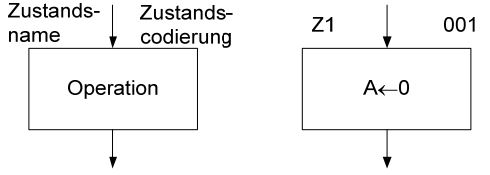
\includegraphics[width=0.8\linewidth]{Zeichnungen/ASM-Zustandsbox}
	  				\end{mytemize}
	  		\end{mytemize}
	  		\begin{mytemize}
	  			\item Entscheidungsboxen
	  				\begin{mytemize}
	  					\item Es wird auf ein Steuersignal reagiert
	  					\item je nach Zustand des Signals (0 oder 1) wird der entsprechende Pfad gewählt
	  					\item 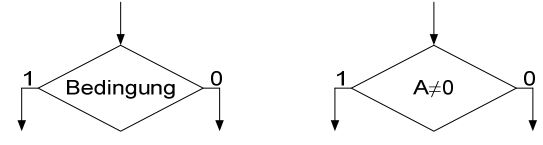
\includegraphics[width=0.8\linewidth]{Zeichnungen/ASM-Entscheidungsbox}
	  				\end{mytemize}
	  		\end{mytemize}
		  	\begin{mytemize}
		  		\item Bedingte Zustandsboxen
		  			\begin{mytemize}
		  				\item Ein Zustand kann nur über eine Bedingung erreicht werden
		  				\item 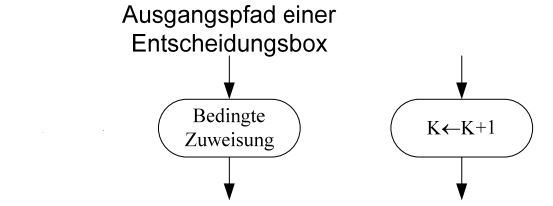
\includegraphics[width=0.8\linewidth]{Zeichnungen/ASM-Bed-Zustandsbox}
		  			\end{mytemize}
		  	\end{mytemize}
	  	\end{mytemize}
	  \end{karsten}
  \item Was ist der Unterschied zwischen einem ASM-Diagramm und einem Flowchart?
  	\begin{karsten}
  		\begin{mytemize}
  			\item Der generelle Aufbau sit der gleiche
  			\item Beim Flowchart finden alle Entscheidungen, Zustandsboxen, etc NACHEINANDER statt
  			\item beim ASM-Diagramm können Entscheidungen und Zustandsboxen innerhalb eines Taktes bearbeitet werden
  		\end{mytemize}
	\end{karsten}
  \item Wie erfolgt die Abbildung eines ASM Diagramms in einen Automaten?
  \item Nennen Sie die Steuerformen für Steuerwerke!
  \item Erklären Sie die One-Hot-Kodierung anhand einer Skizze!
  \item Erklären Sie die Register-Decoder Steuerung anhand einer Skizze!
  \item Wozu wird die Zustandskodierung in einem Steuerwerk benötigt?
        \begin{mytemize}
          \item Warum ist die Wahl der Zustandskodierung von Bedeutung?
          \item Nennen und erklären Sie heuristische Regeln für die Zustandskodierung!
        \end{mytemize}
  \item Erklären sie Mikroprogrammgesteuerte Kontrolle anhand einer Skizze.
  \item Wie funktioniert ein Sequenzer auf Basis eines Mikroprogrammzählers?
        \begin{mytemize}
          \item Wie müssen die zugehörigen Mikroinstruktionen aussehen?
        \end{mytemize}
  \item Erklären Sie
        \begin{mytemize}
          \item horizontale Mikroprogrammierung
                \begin{mytemize}
                  \item Vorteile
                  \item Nachteile
                \end{mytemize}
          \item vertikale Mikroprogrammierung
                \begin{mytemize}
                  \item Vorteile
                  \item Nachteile
                \end{mytemize}
          \item diagonale Mikroprogrammierung
                \begin{mytemize}
                  \item Vorteile
                  \item Nachteile
                \end{mytemize}
        \end{mytemize}
\end{mytemize}

% --------------------------
\subsection*{Mikroprozessor}
% --------------------------
\begin{mytemize}
  \item Was ist ein Mikroprozessor?
        \begin{mytemize}
          \item Aus welchen Komponenten besteht er?
        \end{mytemize}
  \item Erklären Sie die Begriffe
        \begin{mytemize}
          \item Signalprozessor
          \item Mikrocontroller
          \item SoC
        \end{mytemize}
  \item Was ist das Von-Neumann-Prinzip?
  \item Skizzieren Sie einen vollständigen Prozessor mit Operationswerk, mikroprogrammiertem Steuerwerk, Speichereinheiten für Daten und Befehle, einem Befehlsregister (IR), Befehlsdecoder und einer Ein-/Ausgabeeinheit.
  \item Skizzieren Sie das Operationswerk eines Prozessors mit einer ALU, Registern, Decoder und Multiplexern.
  \item Erklären Sie die Verwendung des Decoders und der Multiplexer zur Bereitstellung von Eingabedaten bzw. zum Speichern der Ausgabedaten der ALU!
  \item Was ist das Operationsprinzip der Von-Neumann-Architektur?
  \item Erklären Sie die Begriffe
        \begin{mytemize}
          \item Prozessorarchitektur
          \item Mikroarchitektur
          \item Prozessorfamilie
        \end{mytemize}
  \item Was sind die Bestandteile der Prozessorarchitektur?
  \item Welche Befehlsformate kennen Sie? Geben Sie Beispiele.
  \item Nennen und erklären Sie die Gruppen von Befehlen in einem Befehlssatz. Geben Sie Beispiele für jede Gruppe!
  \item Wie werden Befehlssatz-Architekturen klassifiziert?
  \item Was definiert das Speichermodell einer Prozessorarchitektur?
  \item Welche Speicheradressräume für Daten kennen Sie?
  \item Wie funktioniert ein Stack?
  \item Wie funktioniert implizite Operandenadressierung?
  \item Nennen und erklären Sie die expliziten Adressierungsarten! Geben Sie jeweils ein Beispiel.
  \item Erklären Sie die Realisierung der Adressierungsarten in Hardware anhand einer Skizze!
  \item Erklären Sie RISC (Reduced Instruction Set Computer)!
  \item Wie funktioniert ein Interrupt?
        \begin{mytemize}
          \item Wozu wird dieser benötigt?
        \end{mytemize}
  \item Erklären Sie Daisy Chain! Geben Sie auch eine Skizze.
  \item Erklären Sie Interrupt-Controller! Geben Sie auch eine Skizze mit den Registern im Interrupt-Controller sowie den Signalen zur CPU und zu Interruptquellen.
  \item Erklären Sie die Befehlsausführungphasen
        \begin{mytemize}
          \item \glqq{}Decodierphase\grqq
          \item \glqq{}Ausführungsphase\grqq
        \end{mytemize}
  \item Erklären Sie Pipelining.
        \begin{mytemize}
          \item Welche Anforderungen bestehen für korrekte Exekution bei Pipelining?
        \end{mytemize}
\end{mytemize}

% ------------------------------
\subsection*{Speicherverwaltung}
% ------------------------------
\begin{mytemize}
  \item Was sind die Anforderungen an Speicherverwaltung?
  \item Welche Arten von Speicher in einem Rechnersystem kennen Sie?
        \begin{mytemize}
          \item In welchen Eigenschaften unterscheiden sich diese Speicher?
        \end{mytemize}
  \item Erklären Sie
        \begin{mytemize}
          \item Fixed Partitioning
          \item Dynamic Partitioning
        \end{mytemize}
  \item Was ist Fragmentierung des Speichers?
  \item Erklären Sie Relocation?
  \item Erklären Sie die Adressübersetzung bei relativen Adressen.
        \begin{mytemize}
          \item Zeichnen Sie eine Skizze mit den notwendigen Registern, dem Addierer und Komparator und dem Prozess-Image.
        \end{mytemize}
  \item Wie funktioniert Paging?
        \begin{mytemize}
          \item Geben Sie ein Beispiel für die Adressumsetzung beim Paging!
        \end{mytemize}
  \item Wie funktioniert Segmentierung?
        \begin{mytemize}
          \item Geben Sie ein Beispiel für die Adressumsetzung bei Segmentierung!
        \end{mytemize}
  \item Was ist virtueller Speicher?
        \begin{mytemize}
          \item Erklären Sie Memory Fault
          \item Erklären Sie Trashing
        \end{mytemize}
  \item Wie funktioniert ein Translation Lookaside Buffer?
  \item Erklären Sie den Begriff Fetch Policy!
  \item Erklären Sie den Begriff Replacement Policy, geben und erklären Sie drei Beispiele!
  \item Was ist das Resident Set?
\end{mytemize}

% ---------------------------
\subsection*{Mikrocontroller}
% ---------------------------
\begin{mytemize}
  \item Erstellen Sie eine Zeichnung des Schalenmodells eines Mikrocontrollers!
  \item Wozu werden zeitbasierte Komponenten eines Mikrocontrollers benötigt?
  \item Erklären Sie die Zähler- und Zeitgebereinheit und geben Sie Anwendungsbeispiele!
  \item Erklären Sie die \glqq{}Capture und Compare\grqq-Einheit und geben Sie Anwendungsbeispiele!
  \item Wie funktioniert Pulsweitenmodulation?
  \item Erklären Sie einen Pulsweitenmodulator!
  \item Erklären Sie eine Watchdog-Einheit!
  \item Erklären Sie Echtzeit Ein-/Ausgabeeinheiten!
  \item Was ist der Unterschied zwischen isolierter Adressierung und gemeinsamer Adressierung zur Anbindung des E/A-Adressraums an den Prozessorkern?
  \item Erklären Sie digitale parallele Ein-/Ausgabeeinheiten!
  \item Erklären Sie digitale serielle Ein-/Ausgabeeinheiten!
  \item Wie funktioniert asynchrone und synchrone Übertragung?
  \item Erklären sie das Serial Peripheral Interface!
  \item Erklären Sie die Übertragungscodes
        \begin{mytemize}
          \item NRZ
          \item Manchester
          \item MFM
          \item Geben Sie Beispiele!
        \end{mytemize}
  \item Wie kann der Ausgleich von Geschwindigkeitsunterschieden zwischen E/A und Prozessorkern erfolgen?
  \item Erklären Sie die Analog/Digital-Wandlung und Digital/Analog -Wandlung anhand eines Funktionsgraphen (horizontale Achse: digitaler Wert zwischen 0 und $2^{n-1}$, vertikale Achse: analoger Spannungswert)!
  \item Was sind die wichtigsten Kriterien für die Auswahl eines Wandlers?
  \item Nennen und erklären Sie die Wandlungsfehler!
  \item Wie funktioniert das Wägeverfahren zur Analog/Digital-Wandlung?
  \item Welche Fehler gibt es bei der Analog/Digital Wandlung zusätzlich zu den Fehlern der D/A-Wandlung?
  \item Erklären Sie den Ablauf eines DMA Transfers und den Ablauf eines Datentransfers per Software!
  \item Was ist der Unterschied zwischen Fly-By-Transfer und Two-Cycle-Transfer?
  \item Skizzieren Sie den Aufbau eines DMA-Controllers!
  \item Was ist
        \begin{mytemize}
          \item Einzeltransfer?
          \item Blocktransfer?
          \item Demand Transfer?
        \end{mytemize}
  \item Erklären Sie
        \begin{mytemize}
          \item Daten-Multiplexing bei einem Erweiterungsbus
          \item Daten/Adress-Multiplexing bei einem Erweiterungsbus
        \end{mytemize}
  \item Was ist ein Burst-Transfer?
  \item Geben Sie eine Formel für die elektrische Leistung in CMOS Schaltungen an und benennen Sie die verschiedenen Größen!
  \item Wie ist der Zusammenhang zwischen Spannung und Taktfrequenz in einer Schaltung?
  \item Wie ist der Zusammenhang zwischen elektrischer Leistung und Spannung/Taktfrequenz?
  \item Wie funktioniert Dynamic Voltage Frequency Scaling?
\end{mytemize}

% ------------------------------------------------------------------------------
\end{document}
% ------------------------------------------------------------------------------

